\chapter{Numerical Simulation}
\label{chp_Num_sim}

\section{Introduction}
To grasp the ESG-swap rate process $\kappa_{t}^{ESG}$, we need a model for the ESG-risk score process of the company. It could be logical with a downward trending score since the company will be incentivised to enter such an agreement. 
\\~\\
There are many possible alternatives to model such a model, so we impose the following model for the \textbf{ESG-risk score}:
\[
X(t) = 100\exp(-Z(t))
\]

Here $Z(t)$ is an OU-process
\nomenclature{OU}{Ornstein Uhlenbeck}
given by: 
\begin{align*}
dZ(t) &= -\beta Z(t)dt + \sigma dW^{Q}(t) + dI^{Q}(t)    
\end{align*} 
Where: 
\begin{align*}
I^{Q}(t) &= \sum_{k=1}^{N(t)}J_{k}, \;\; J_{k}\sim Exp(\mu),\;\; N(t) \sim Pois(\lambda t)    
\end{align*} 

Furthermore $I^{Q}$ and $W^{Q}$ are assumed to be independent, now for $J\sim Exp(\mu)$, we have:
\begin{align*}
f_{J}(x) &= \mu e^{-\mu x}\mathbbm{1}_{[0,\infty)}(x), \;\; 
\E[J] = \frac{1}{\mu}, \;\text{and}\; Var[J] = \frac{1}{\mu^{2}}
\end{align*}

An explicit solution is given by: 
\begin{align}
\label{eq: characteristic_function_Z(t)}
d[e^{\beta t}Z(t)] &= d[e^{\beta t}]Z(t) + e^{\beta t}dZ(t) \nonumber \\ 
&= \beta e^{\beta t}Z(t)dt + e^{\beta t}[-\beta Z(t)dt + 
\sigma dW^{Q}(t) + dI^{Q}(t)]
\nonumber \\ 
&=\sigma e^{\beta t}dW^{Q}(t) + e^{\beta t}dI^{Q}(t) \nonumber \\ 
&\Downarrow \nonumber\\ 
Z(t) &= Z(0)e^{-\beta t} +
\int_{0}^{t}e^{-\beta (t-s)}dW^{Q}(s) + 
\int_{0}^{t}e^{-\beta (t-s)}dI^{Q}(s)
\end{align} 



\newpage 

\begin{proposition}[\textbf{Characteristic function of $Z(t)$}]
\label{prop: Characteristic_function_ESG_risk_score}
The characteristic function of $Z(t)$ is given by:
\begin{align*}
\E_{Q}\left[
\exp(iu Z(t))
\right] 
&= 
\exp\left(
iuZ(0)e^{-\beta t}\right)
\left(
-\frac{u^{2}}{4\beta}[1-e^{-2\beta t}]
\right)
\left(
\frac{
1-iue^{-\beta t}1/\mu}
{
1-iu1/\mu
}
\right)^{\frac{\lambda}{\beta}}    
\end{align*}
\end{proposition}

\begin{proof}
Since $I^{Q}$ and $W^{Q}$ are independent we have that: 
\begin{align*}
\E_{Q}[e^{iuZ(t)}]
&= 
\exp\left(
iuZ(0)e^{-\beta t}
\right)
\E_{Q}\left[
\exp\left(
iu\int_{0}^{t}e^{-\beta(t-s)}dW^{Q}(s)
\right)
\right]
\E_{Q}\left[
\exp\left(
iu\int_{0}^{t}e^{-\beta(t-s)}dI^{Q}(s)
\right)
\right]
\end{align*}

The normality of deterministic Ito-integrals gives us the following:
\begin{align*}
iu\int_{0}^{t}e^{-\beta(t-s)}dW^{Q}(s) &\sim \mathcal{N}\left(
0, -u^{2}\int_{0}^{t}e^{-2\beta(t-s)}ds
\right) \\ 
&\Downarrow \\ 
\E_{Q}\left[
\exp\left(
iu\int_{0}^{t}e^{-\beta(t-s)}dW^{Q}(s)
\right)
\right]
&= 
\exp\left(
-\frac{u^{2}}{4\beta}[1-e^{-2\beta t}]
\right)
\end{align*}

From Proposition \ref{prop: Integral_g(s)dI(s)} p.\pageref{prop: Integral_g(s)dI(s)}, we have: 
\begin{align*}
\E\left[
\exp\left(iu\int_{0}^{t}e^{-\beta(t-s)}dI(s)\right)
\right] 
&= 
\exp\left(
\int_{0}^{t}\Psi(ue^{-\beta s})ds
\right)
\end{align*}

To ease some notation, we write:
\begin{align*}
\Psi(x) &= \lambda(\varphi_{F}(x) - 1), \;\text{where:}\; 
\varphi_{F}(x) = \int_{\R}e^{iyx}F_{J}(dy) 
\end{align*}

We start with calculating $\varphi_{F}(x)$ with $F_{J}(dy) = 
\mu e^{-\mu y}\mathbbm{1}_{[0,\infty)}(y)dy:$ 
\begin{align*}
\varphi_{F}(x) &= 
\int_{0}^{\infty}e^{ixy}\mu e^{-\mu y}dy   
= \frac{1}{1-ix\frac{1}{\mu}}
\end{align*}

Giving us:
\begin{align*}
\varphi_{F}(x) - 1
= 
\frac{1}{1-ix\frac{1}{\mu}} - \frac{1-ix\frac{1}{\mu}}{1-ix\frac{1}{\mu}} 
= 
\frac{ix\frac{1}{\mu}}{1-ix\frac{1}{\mu}}
\end{align*}

Now: 
\begin{align*}
\Psi(ue^{-\beta s}) &= \lambda(\varphi_{F}(ue^{-\beta s})) -1) \\ 
&= \lambda\left(
\frac{iue^{-\beta s}1/\mu}{1-iue^{\beta s}1/\mu}
\right)\cdot \frac{\beta}{\beta} \\ 
&= 
\frac{\lambda}{\beta}\left(
\frac{\beta iue^{-\beta s}1/\mu}{1-iue^{\beta s}1/\mu}
\right)
\end{align*}

\newpage 
We observe: 
\begin{align*}
h(s) :&= \ln[1-iue^{-\beta s}1/\mu] \\ 
&\Downarrow \\ 
h'(s) &= \frac{\beta iue^{-\beta s}1/\mu}{1-iue^{\beta s}1/\mu} 
\end{align*}

Leaving us with: 
\begin{align*}
\int_{0}^{t}\Psi(ue^{-\beta s})ds
&= 
\frac{\lambda}{\beta}\int_{0}^{t}h'(s)ds
= 
\frac{\lambda}{\beta}[h(t)-h(0)] 
= 
\frac{\lambda}{\beta}
\ln\left[
\frac{1-iue^{-\beta t}1/\mu}{1-iu1/\mu}
\right]
\end{align*}

\end{proof}


By using Proposition \ref{prop: Characteristic_function_ESG_risk_score} we can find the expectation of $X(t)$: 
\begin{align*}
\E_{Q}\left[X(t)\right]
&= 
\E_{Q}\left[
e^{i(-i)Z(t)}
\right] \\ 
&= 
\exp\left(
Z(0)e^{-\beta t}
\right)
\exp\left(
\frac{1}{4\beta}[1-e^{-2\beta t}]
\right)
\left(
\frac{
1 + e^{-\beta t}1/\mu
}{
1 + 1/\mu
}
\right)
\end{align*}

Now if $\beta > 0$, one can find: 
\begin{align*}
\lim\limits_{t \to \infty}\E_{Q}[X(t)]
&= 
\exp\left(
\frac{1}{4\beta} + \frac{1}{1+1/\mu}
\right)
\end{align*}

\begin{figure}[htp]
    \centering
    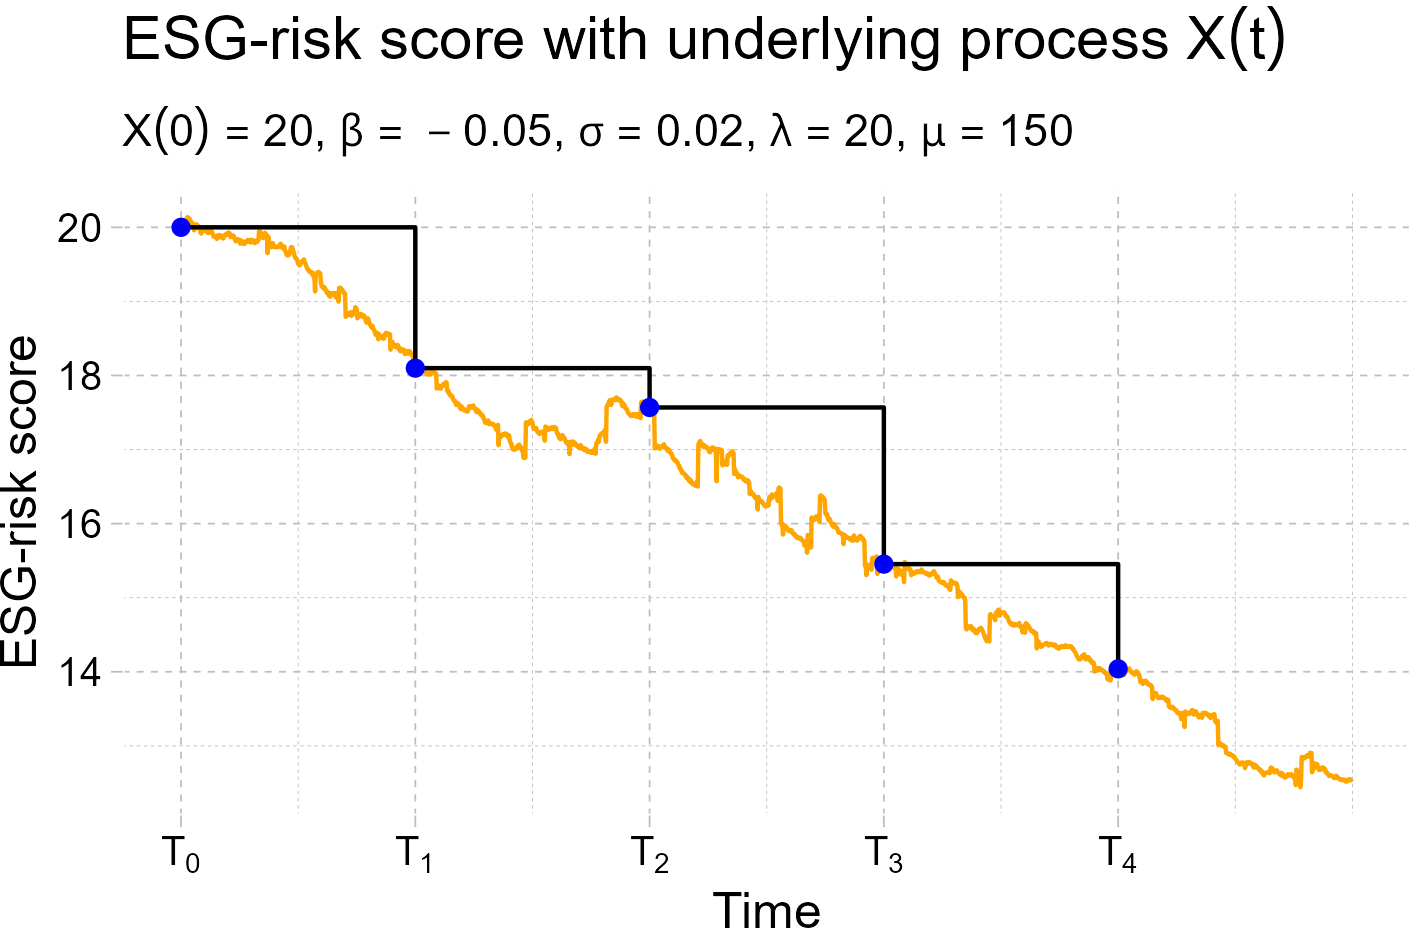
\includegraphics[width=11cm]{figures/ESG/ESG_OU_path.png}
    \caption{ESG-risk score with underlying process $X(t)$}
    \label{fig: ESG_risk_score_underlying_X(t)}
\end{figure}

The blue dots represent the observed ESG-risk score at the relevant observation times. The solid dark line represents the ESG-risk score between observation times, and the underlying orange process describes our continuous time ESG-risk score process $X(t)$.  

\newpage 

\section{Simulation of Zero Coupon Bond ESG-swap}

In this section, we will look at a numerical simulation of the ESG-swap rate process $\kappa_{t}^{ESG} = (\kappa_{t}^{ESG}(i))_{i=1, \dots, 4}$. We will simulate different scenarios. These will be when the ESG-criteria $C^{ESG}$ is reasonable and when the ESG criteria are unreasonable. 
\\~\\
By unreasonable, we will look at the extremes, i.e. where the criteria are met all the time and where the criteria are never satisfied. This will show the effect of the discount and penalty, respectively. 
\\~\\ 
After analysis, one has concluded that the model described in Figure \ref{fig: ESG_risk_score_underlying_X(t)} is a good fit for the counterparty company in this ESG swap. 
\\~\\
\textbf{Parameters}
\begin{itemize}
    \item $X(0) = 20 \implies Z(0) = -\ln\left(\frac{20}{100}\right)$
    \item $\beta = -0.05$
    \item $\sigma = 0.02$
    \item $\lambda = 20$
    \item $\mu = 150$
\end{itemize}

We will use a stepsize of $dt = \frac{1}{360}$, and since the calculation is based upon Monte Carlo simulations, we will establish the analysis on 1 Million simulations. 
\\~\\ 
\textbf{Agreement/specifications}
\begin{itemize}
    \item For simplicity, we will assume that our ESG criteria process $C^{ESG} = (C^{ESG}_{T_{i}})_{
    \{i=1, \dots, 4\}}$ to be $\F_{0}$-measurable. 
    \item $\delta = 1$ meaning that the time between observations times $T_{i}$ and $T_{i-1}$ is one year. 
    \item We assume that the penalty/discount $d = 0.005$.
    \item We will also, for simplicity, set: 
    \[
    \kappa_{t}^{ZCB} = \frac{P(t,T_{0})-P(t,T_{4})}{\delta \sum_{i=1}^{4}P(t,T_{i})} = 0.07
    \]
\end{itemize}
\newpage 

\textbf{Reasonable criteria}
\begin{itemize}
    \item $C^{ESG} = (17.8, 16.8, 15.8, 14.8)$
\end{itemize}

\begin{figure}[htp]
    \centering
    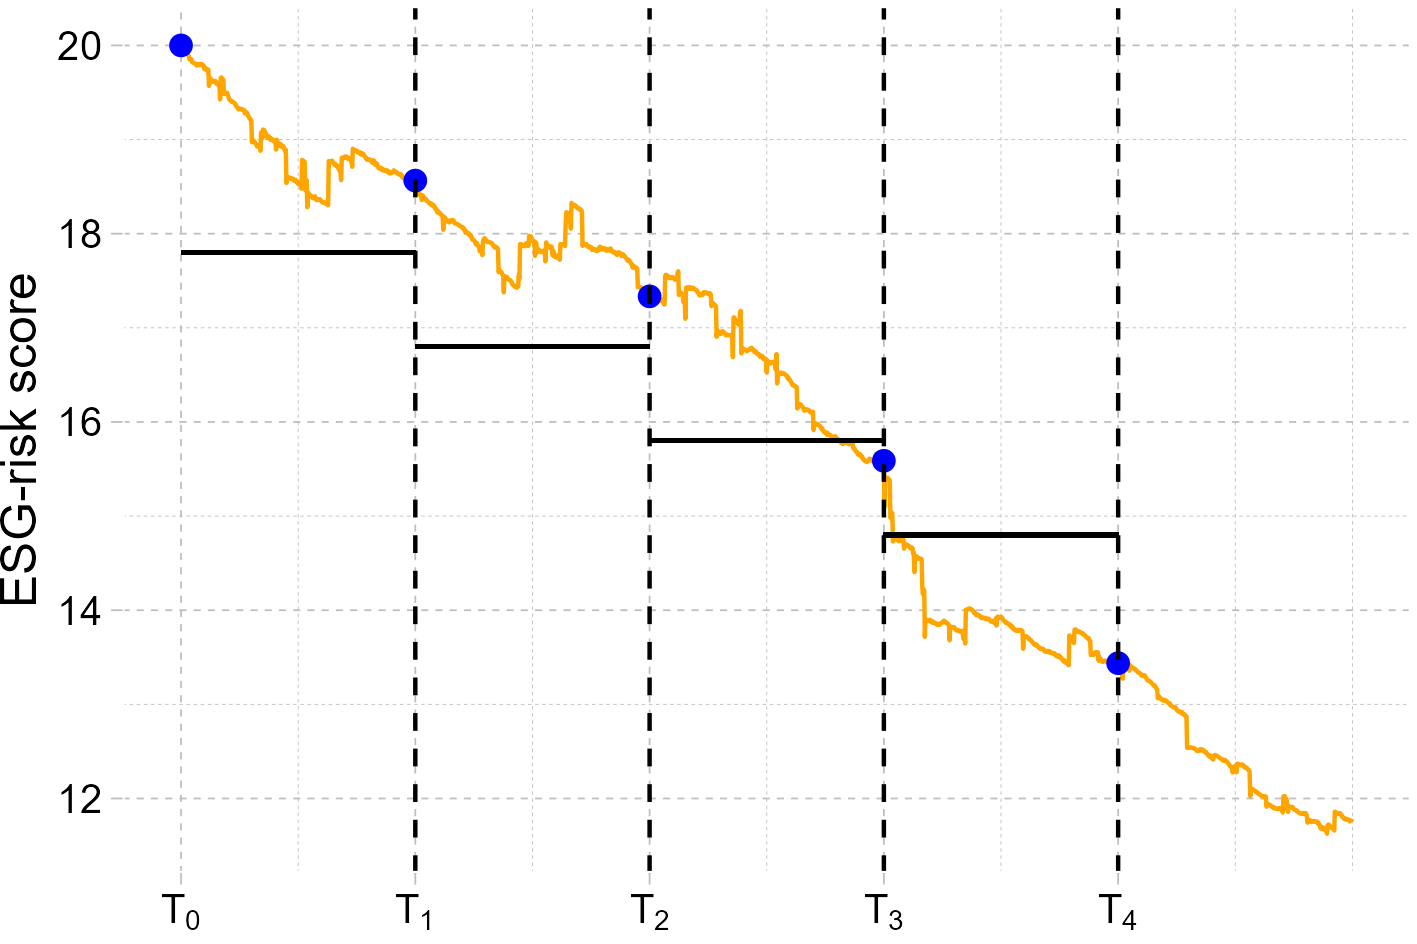
\includegraphics[width= 9cm]{figures/ESG/ESG_plt_criteria1.png}
    \caption{ESG-risk score where ESG-criteria is reasonable}
    \label{fig: ESG_risk_criteria1}
\end{figure}

In this figure, we see the underlying ESG risk score process. Here the dark-solid lines represent the criteria $C_{T_{i}}^{ESG}$. The blue dots represent the ESG-risk score at time $T_{i}$.
In this particular realization, we see that the criteria are not met at $T_{1}$ and $T_{2}$, and then met at $T_{3}$ and $T_{4}$. 
\\~\\ 
After 1 Million simulations, we got:
\\~\\
\begin{center}
\begin{tabular}{lcccl}
\toprule
           &$C_{T_{i}}^{ESG}$ & $\kappa_{t}^{ZCB}$  & $\kappa_{t}^{ESG}$ \\
\midrule
$T_{1}$ &  17.8 & 0.070 & 0.071 \\
$T_{2}$ &  16.8 & 0.070 & 0.070 \\
$T_{3}$ &  15.8 & 0.070 & 0.068 \\
$T_{4}$ &  14.8 & 0.070 & 0.065 \\
\bottomrule
\end{tabular}
\end{center}

\begin{figure}[htp]
    \centering
    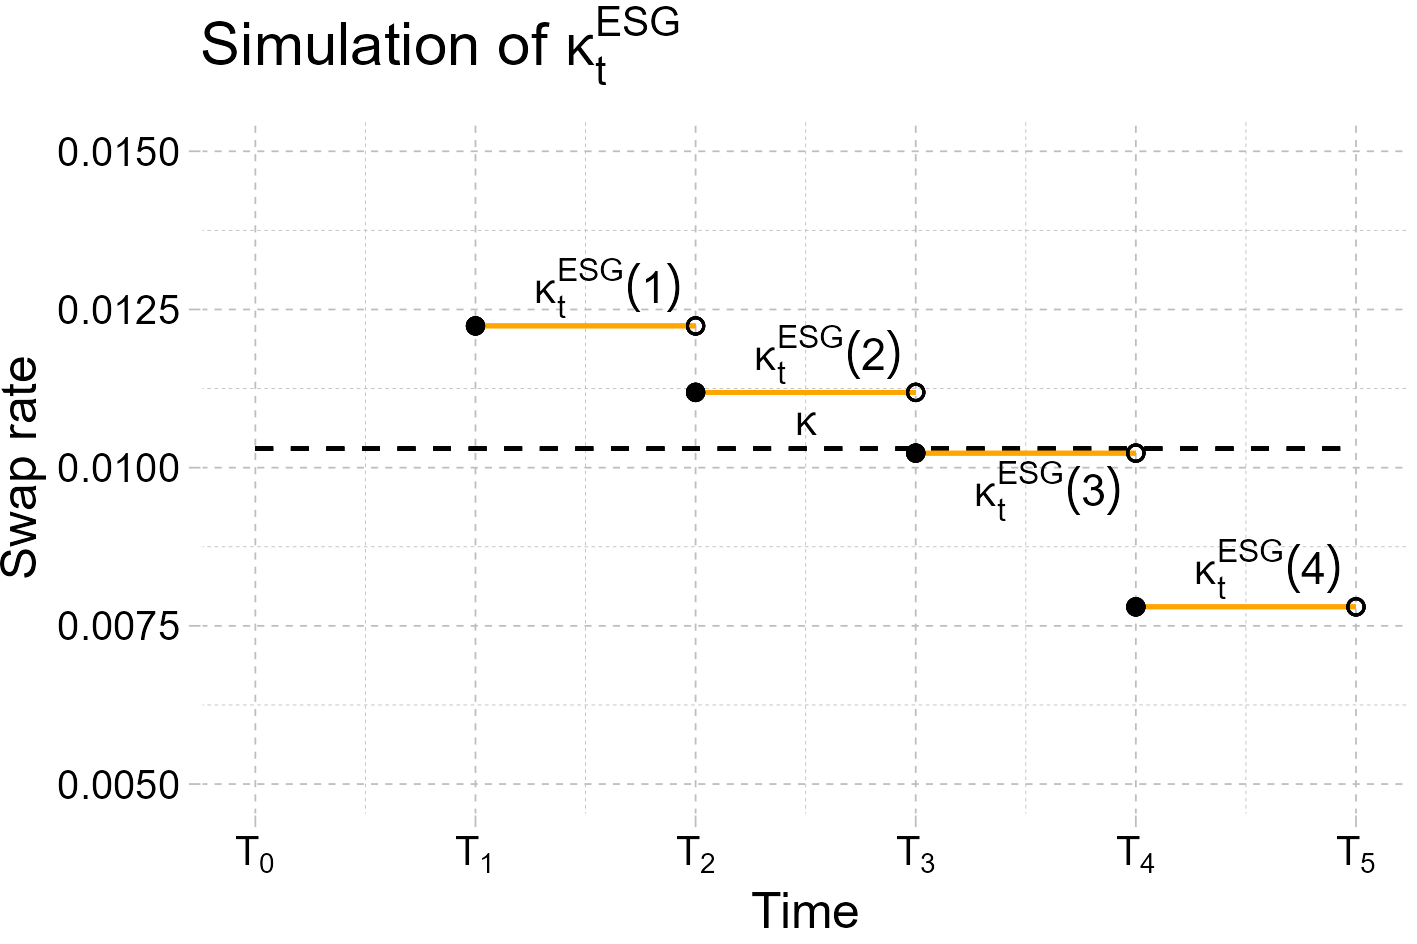
\includegraphics[width= 9cm]{figures/ESG/kappa_t_ESG_1.png}
    \caption{ESG-swap rate when ESG-criteria is reasonable}
    \label{fig: ESG_swap_1}
\end{figure}

\newpage 
\textbf{unreasonable criteria, where criteria are always met}
\begin{itemize}
    \item $C^{ESG} = (24,23,22,21)$
\end{itemize}

\begin{figure}[htp]
    \centering
    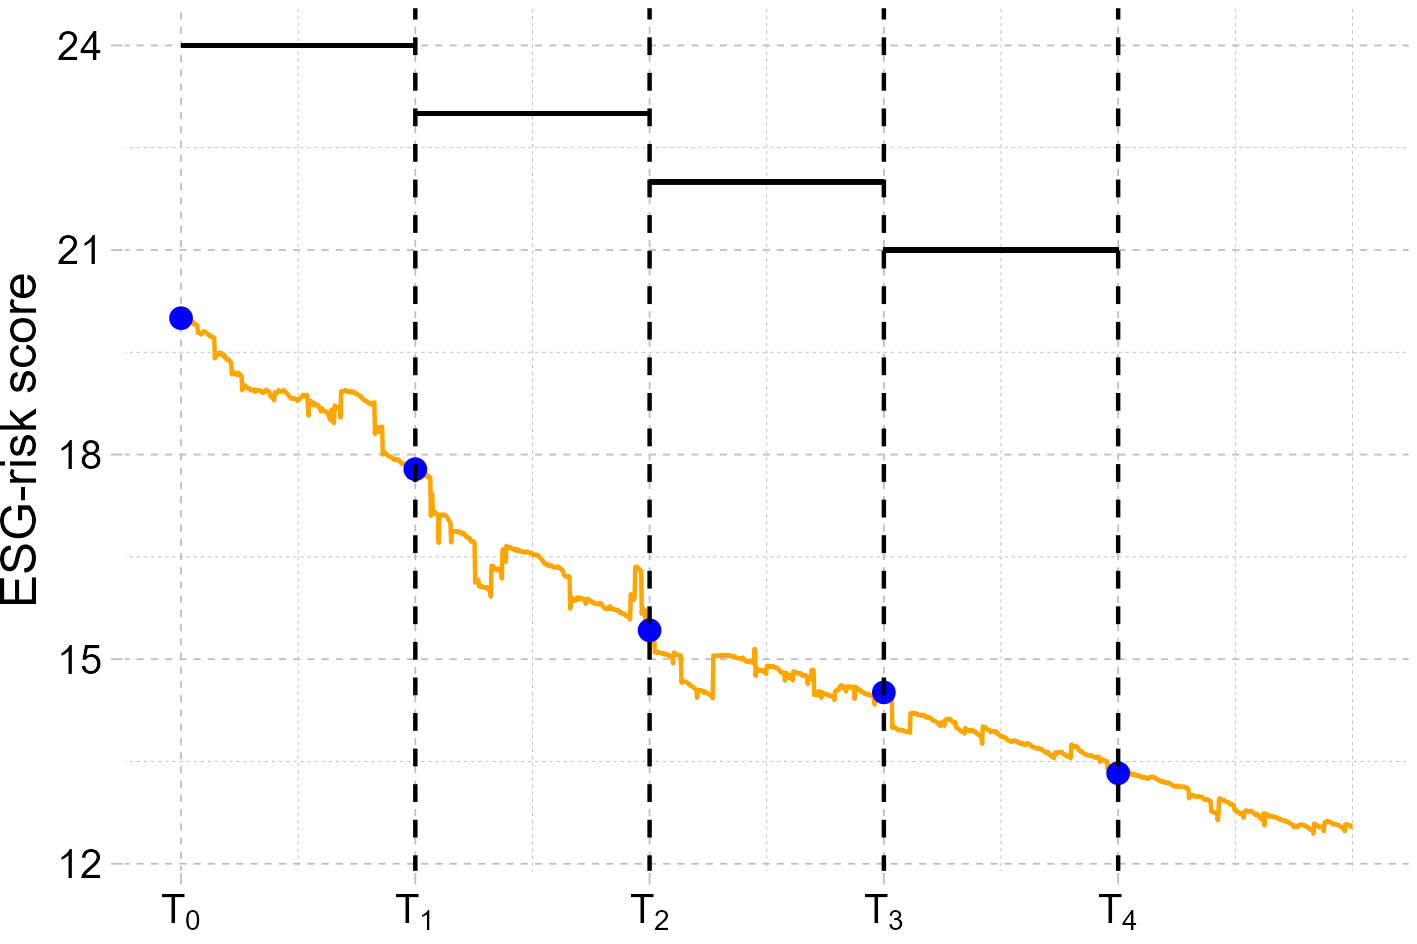
\includegraphics[width= 10cm]{figures/ESG/ESG_plt_criteria2.png}
    \caption{ESG-risk score where ESG-criteria is unfavourable for lender}
    \label{fig: ESG_risk_criteria_2}
\end{figure}

The blue dots are always under the dark solid lines, meaning the criteria are always met.
\\~\\ 
After 1 Million simulations, we got:
\\~\\
\begin{center}
\begin{tabular}{lcccl}
\toprule
           &$C_{T_{i}}^{ESG}$ & $\kappa_{t}^{ZCB}$  & $\kappa_{t}^{ESG}$ \\
\midrule
$T_{1}$ &  24 & 0.070 & 0.065 \\
$T_{2}$ &  23 & 0.070 & 0.060 \\
$T_{3}$ &  22 & 0.070 & 0.055 \\
$T_{4}$ &  21 & 0.070 & 0.050 \\
\bottomrule
\end{tabular}
\end{center}


\begin{figure}[htp]
    \centering
    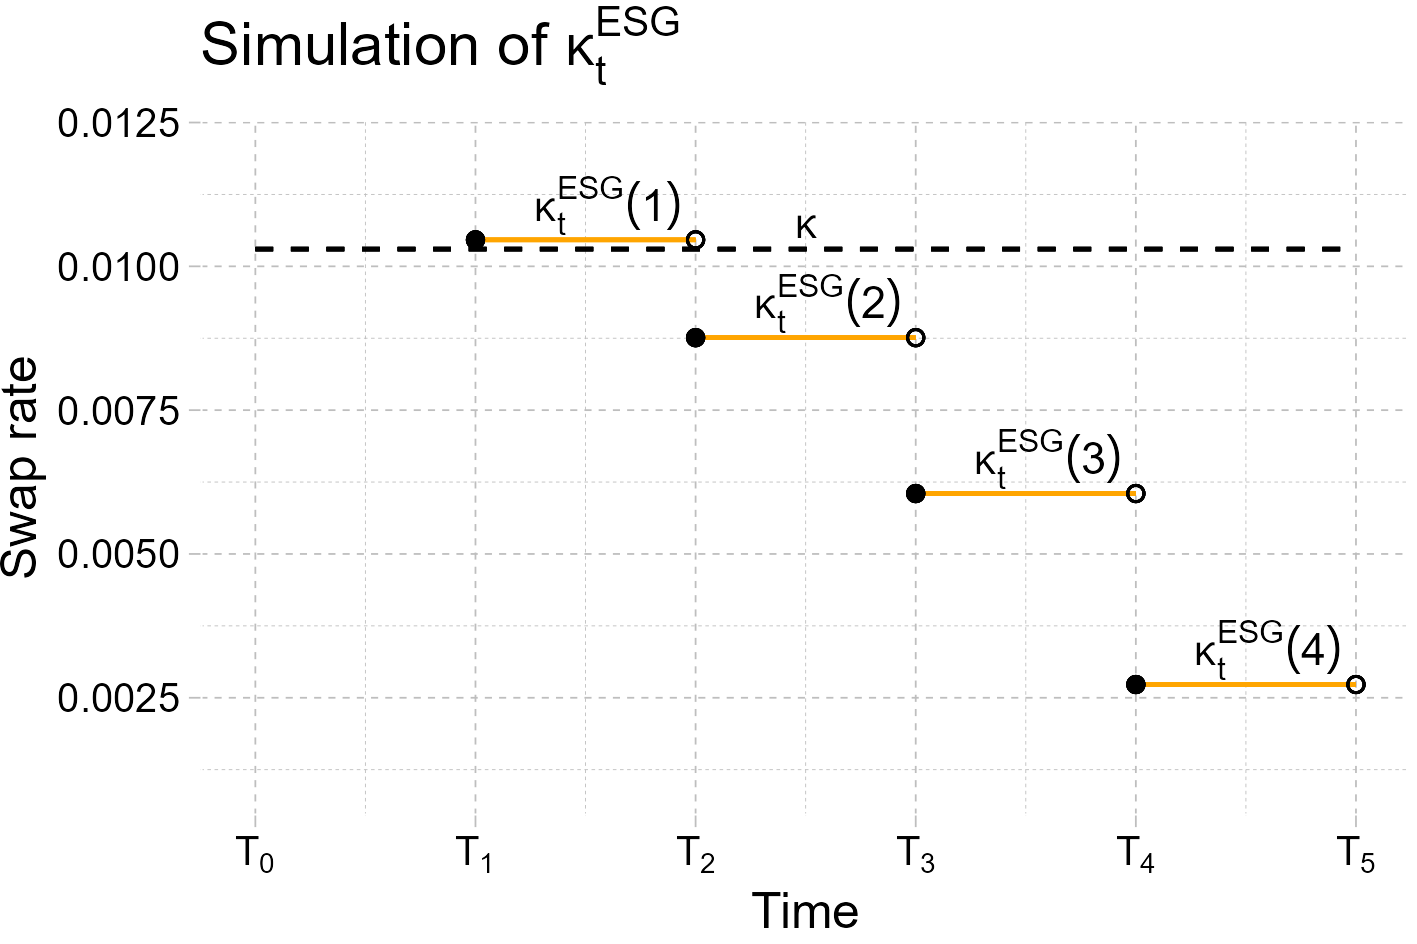
\includegraphics[width= 9cm]{figures/ESG/kappa_t_ESG_2.png}
    \caption{ESG-swap rate, when ESG-criteria is not reasonable for the lender}
    \label{fig: ESG_swap_2}
\end{figure}

Here we see the effect of how the discount $d$ works. For each $T_{i}$, we see that $\kappa_{t}^{ESG}$ goes down by the discount $d$. 

\newpage 
\textbf{unreasonable criteria, where criteria are never met}
\begin{itemize}
    \item $C^{ESG} = (15, 14, 13, 12)$
\end{itemize}

\begin{figure}[htp]
    \centering
    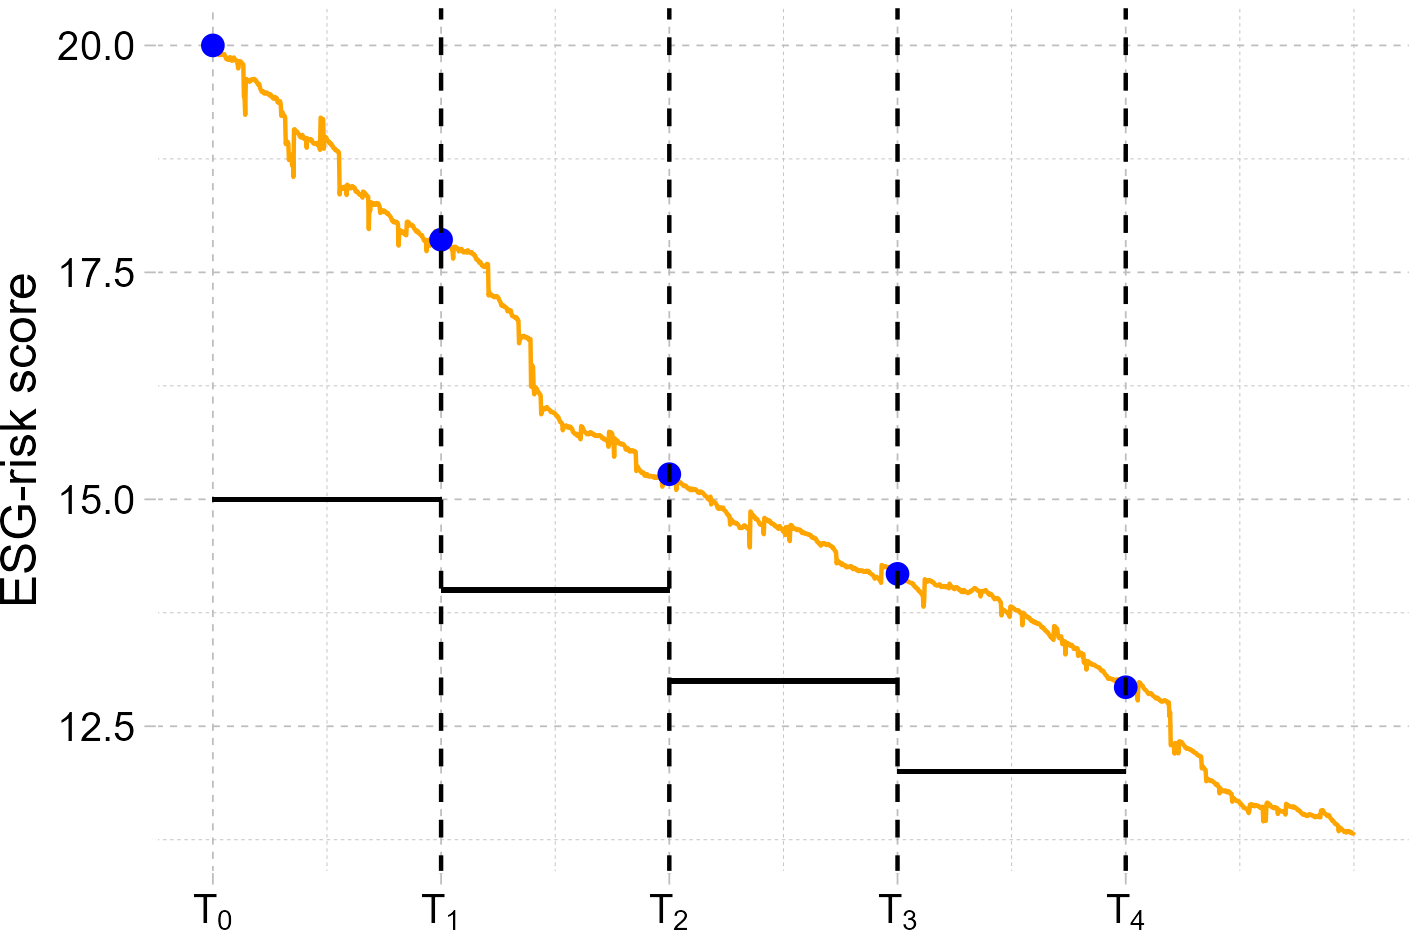
\includegraphics[width= 10cm]{figures/ESG/ESG_plt_criteria3.png}
    \caption{ESG-risk score where ESG-criteria is unfavourable for borrower}
    \label{fig: ESG_risk_criteria_3}
\end{figure} 

The blue dots are consistently above the criteria, meaning that the criteria will not be met. 
\\~\\ 
After 1 Million simulations, we got:
\\~\\
\begin{center}
\begin{tabular}{lcccl}
\toprule
           &$C_{T_{i}}^{ESG}$ & $\kappa_{t}^{ZCB}$  & $\kappa_{t}^{ESG}$ \\
\midrule
$T_{1}$ &  24 & 0.070 & 0.075 \\
$T_{2}$ &  23 & 0.070 & 0.080 \\
$T_{3}$ &  22 & 0.070 & 0.085 \\
$T_{4}$ &  21 & 0.070 & 0.090 \\
\bottomrule
\end{tabular}
\end{center}

\begin{figure}[htp]
    \centering
    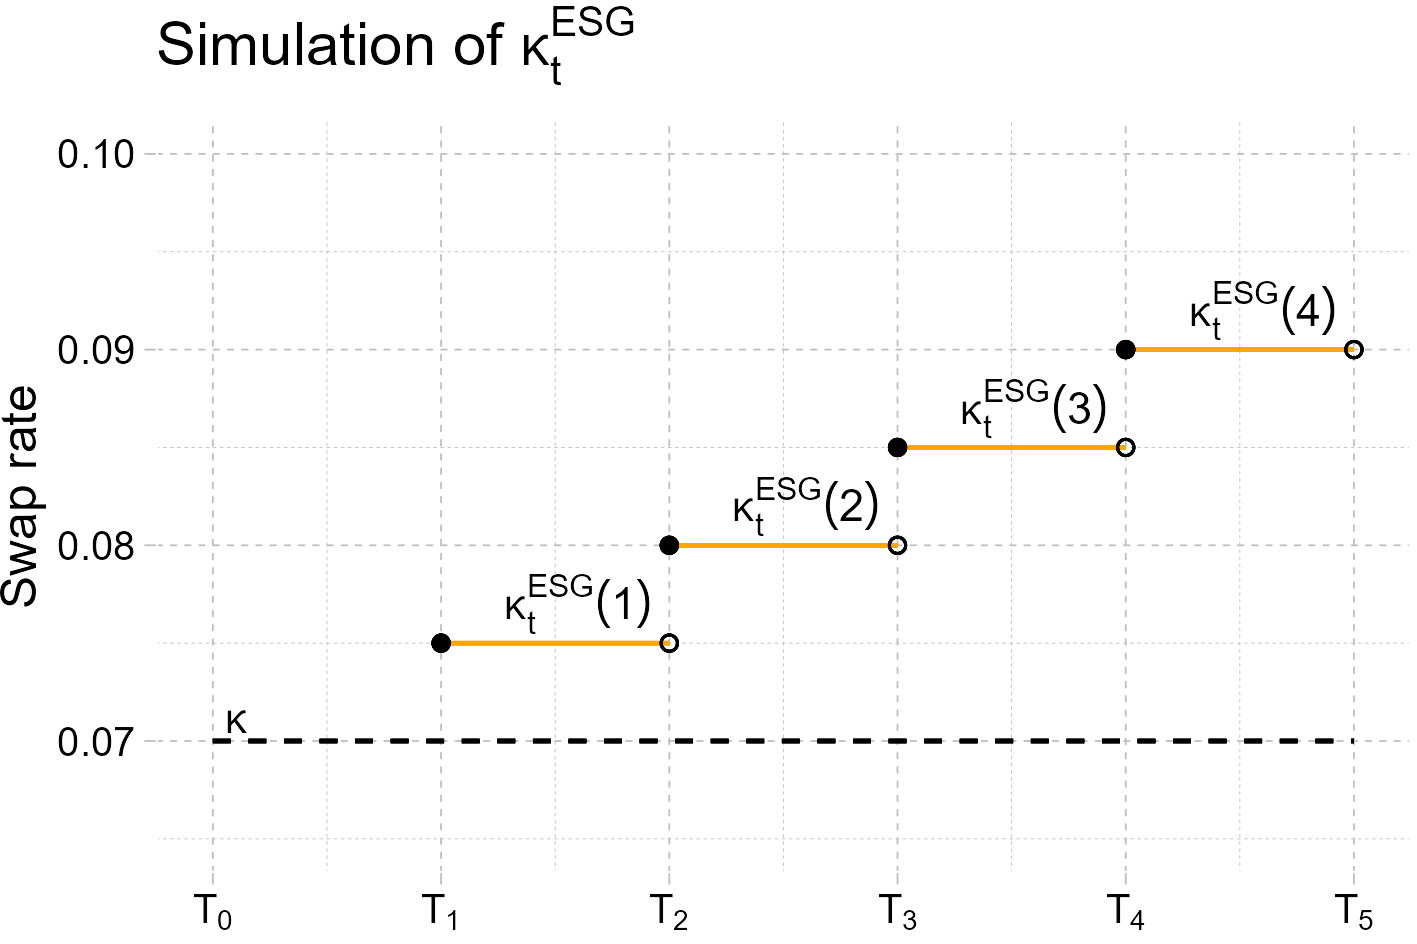
\includegraphics[width= 10cm]{figures/ESG/kappa_t_ESG_3.png}
    \caption{ESG-swap rate, when ESG-criteria is not reasonable for the borrower}
    \label{fig: ESG_swap_3}
\end{figure}

In this situation, $d$ works like a penalty, and correspondingly $\kappa_{t}^{ESG}$ increases. 

